
\section{Introduction\label{introduction}}


\subsection {Universal Schema}
The goal of automatic knowledge base construction (AKBC) is to build a structured knowledge base (KB) of facts using a noisy corpus of raw text evidence, and perhaps an initial seed KB to be augmented~\citep{NELL,yago,freebase}. AKBC supports downstream reasoning at a high level about extracted entities and their relations, and thus has broad-reaching applications to a variety of domains.
An effective approach to AKBC is Universal Schema.
Universal Schema embeds textual patters and knowledge bases into a shared space in order to reason over relations and entity pairs.
A low dimensional embedding is learned for each entity pair and each relation type using matrix factorization.
The model is then able to infer relations between entities as the dot product between the two entity pair and relation type vectors.

Unfortunately, this formulation limits the generalization of the model.
In its original form, Universal Schema can only reason about entity pairs and textual relations explicitly seen at training time.

\subsection {Compositional Universal Schema}

Recently Universal Schema has been extended to deal with compositional representations of textual relations \citep{toutanova2015representing,verga2015multilingual}
Compositional Universal Schema has two main advantages over explicit modeling of textual patterns.
The first is tt allows for the model to share statistics between very similar patterns.
Instead of modeling the text pattern 'lives in the city' and 'lives in the city of' as distinct atomic units, they can instead be composed compositionally of the same word embeddings.
Second, and even more importantly, Compositional Universal Schema allows us to generalize to all possible textual patterns, allowing us to reason over any arbitrary text.

\begin{figure}[h]
\caption{Top : Universal Schema expresses each textual pattern as an atomic unit \protect\citet{riedel2010modeling}.
Bottom : Compositional Universal Schema uses an lstm to encode each textual relation \protect\cite{verga2015multilingual}. }
\centering
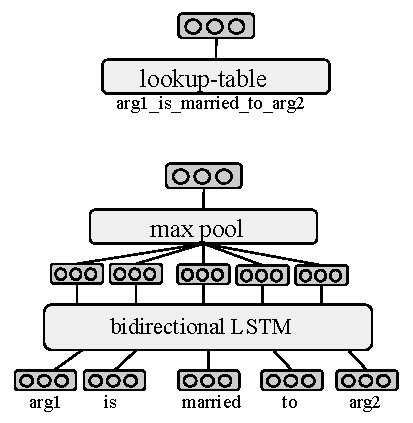
\includegraphics[scale=.68]{relation-models}
\end{figure}

\subsection {Universal Schema without Entity Embeddings}

While Compositional Universal Schema addresses reasoning over arbitrary textual patterns, it is still limited to reasoning over entity pairs seen at training time.
\citet{verga2015multilingual} approach this problem by using Universal Schema as a sentence classifier - directly comparing a textual relation to a kb relation to perform relation extraction.
However, this approach is unsatisfactory for two reasons.
The first is that this creates an inconsistency between training and testing, as the model is trained to predict compatibality between entity pairs and relations and not relations directly.
Secondly, it considers only a single piece of evidence while making its prediction.

The learned entity pair can be seen as a sumamrization of all relations for which that entity pair was seen.


Rather than modeling each entity pair as an explicit vector, we instead treat each entity pair as an aggregate function over each of its relation types.
This allows us to trivially extend to unseen entity pairs, have a direct link to provenance, and allocate a variable number of parameters per entity pair.


\subsection {Entities vs Entity Pairs}

A knowledge base is naturally described as a graph, in which entities are nodes and relations are labeled edges~\citep{yago,freebase}.
In the case of \emph{knowledge graph completion}, the task is akin to link prediction, assuming an initial set of (\emph{s, r, o}) triples.
See~\citet{nickel2015review} for a review.
No accompanying text data is necessary, since links can be predicted using properties of the graph, such as transitivity.
In order to generalize well, prediction is often posed as low-rank matrix or tensor factorization.
A variety of model variants have been suggested, where the probability of a given edge existing depends on a multi-linear form~\citep{rescal,DBLP:journals/corr/Garcia-DuranBUG15,bishan,transe,wang2014knowledge,lin2015learning}, or non-linear interactions between $s$, $r$, and $o$~\citep{socherkb}.

These models all operate at the level of entities rather than entity pairs.
Entity-based models have recall advantages over entity pairs.
For any two entities, the model is able to make predictions even if there is no information regarding the explicit entity pair.
However, this essentially reduces to type clustering as every action star would have a high probability for every action movie.

Entity pairs on the other hand have higher precision.
Both~\citet{toutanova2015representing} and~\citet{limin} observed that the entity pair model outperforms entity models in cases where the entity pair was seen at training time.
This is particularly important when jointly embedding text and knowledge bases.
By leveraging large amounts of unlabeled text, Universal Schema is able to find additional textual evidence for entity pairs.
We are interested in high precision information extraction from direct textual provenance.
